\documentclass{article}


\usepackage{PRIMEarxiv}

\usepackage[utf8]{inputenc} % allow utf-8 input
\usepackage[T1]{fontenc}    % use 8-bit T1 fonts
\usepackage{hyperref}       % hyperlinks
\usepackage{url}            % simple URL typesetting
\usepackage{booktabs}       % professional-quality tables
\usepackage{amsfonts}       % blackboard math symbols
\usepackage{nicefrac}       % compact symbols for 1/2, etc.
\usepackage{microtype}      % microtypography
\usepackage{lipsum}
\usepackage{fancyhdr}       % header
\usepackage{graphicx}       % graphics
\usepackage{color} % Required for yellow background
\usepackage{soul}  % Required for the \hl command
\graphicspath{{media/}}     % organize your images and other figures under media/ folder
\usepackage[numbers]{natbib}   % to make url/doi to appear in bibliography
\usepackage{xcolor}
\newif\ifreview \reviewtrue        % set \reviewfalse for a clean build
\ifdefined\cleanbuild \reviewfalse \fi   % scripts/build_paper.sh --clean defines \cleanbuild
\newcommand{\rev}[1]{\ifreview\textcolor[HTML]{0B5FA5}{#1}\else#1\fi}
\newcommand{\revwhy}[1]{\ifreview\marginpar{\footnotesize\raggedright\textcolor[HTML]{0B5FA5}{#1}}\fi}
\ifreview\setlength{\marginparwidth}{0.85in}\setlength{\marginparsep}{0.08in}\fi


%Header
\pagestyle{fancy}
\thispagestyle{empty}
\rhead{ \textit{ }} 

% Update your Headers here
\fancyhead[LO]{DegradX: A Dataset-Calibrated Synthetic Benchmark for Attribution Evaluation on Degrading Systems}
% \fancyhead[RE]{Firstauthor and Secondauthor} % Firstauthor et al. if more than 2 - must use \documentclass[twoside]{article}



  
%% Title
\title{DegradX: A Dataset-Calibrated Synthetic Benchmark for Attribution Evaluation on Degrading Systems
%%%% Cite as
%%%% Update your official citation here when published 
\thanks{\textit{\underline{Citation}}: 
\textbf{Authors. Title. Pages.... DOI:000000/11111.}} 
}

\author{
  Myroslav Mishchuk \\
  Silesian University of Technology \\ 
  Gliwice, Poland \\
  Lviv Polytechnic National University \\ 
  Lviv, Ukraine \\
  \texttt{myroslav.mishchuk@polsl.pl} \\
   \And
  Rafał Cupek \\
  Silesian University of Technology \\ 
  Gliwice, Poland\\
  \texttt{rafal.cupek@polsl.pl} \\
    \And
  Olena Pavliuk \\
  Silesian University of Technology \\ 
  Gliwice, Poland \\
  Lviv Polytechnic National University \\ 
  Lviv, Ukraine \\
  \texttt{olena.pavliuk@polsl.pl} \\
}

\begin{document}
\maketitle


\begin{abstract}
\end{abstract}

\keywords{Explainable artificial intelligence \and Feature attribution \and Benchmarking \and Time-series regression \and Prognostics and health
management \and Synthetic data generation}


\section{Introduction}
 
Industrial assets degrade in service: bearings wear, rotating machinery loses efficiency, and battery cells lose capacity. Condition monitoring records this progression, directly or indirectly, in sensor time series, and maintenance policies that act on it are economically consequential. A survey of United States manufacturers estimates the total annual cost of inadequate maintenance at \$222.0 billion and reports that respondents relying more heavily on predictive than on preventive maintenance experienced 18.5\,\% less unplanned downtime and 87.3\,\% fewer defects~\cite{thomas2021}. Data-driven models support the tasks on which such policies depend: detecting incipient faults, estimating the current health state, and predicting the remaining useful life (RUL). Because the resulting decisions are consequential, a numerical estimate is seldom sufficient on its own. Before a model is relied upon, engineers need evidence that it responds to the physical signature of degradation rather than to the incidental structure introduced by the acquisition process or by the composition of the training set, and an estimate that triggers an intervention must be justifiable to those who act on it. Post-hoc attribution is by far the most frequently applied method across manufacturing and industrial cyber-physical systems, as it can be applied to a model that is already trained and operational without altering it~\cite{electronics13173497}.
 
Attribution methods assign a value to each element of an input sequence, representing its contribution to the model's output. Whether such a method is faithful (that is, whether the returned values reflect the model's actual dependence on the input) is a separate question from predictive accuracy: a model may estimate its target well while the attribution computed for it misidentifies which inputs drove the estimate. Evaluation of faithfulness requires attribution ground truth specifying the actual contribution of each input element, and on measured data, no such ground truth exists. Validation therefore proceeds by perturbing input elements in order of estimated importance and measuring the effect on model performance. However, the reliability of this procedure is contested at several levels. Occluding elements skew the input distribution, so the model is queried on samples unlike those it was trained on, which is among the drawbacks that motivated dedicated evaluation frameworks for time series~\cite{turbe2023}. Still, such frameworks have themselves since been shown to contain significant weaknesses~\cite{serramazza2024}. The metric commonly used in region perturbation, the Area Under Perturbation Curve (AUPC), was shown to be inadequate on its own for estimating faithfulness and can support incorrect conclusions, revealing neither how well relevant and irrelevant elements are separated nor how consistently, with results depending materially on the perturbation method applied and region size selection~\cite{simic2025}. Under controlled conditions with known relevant elements, the disagreement is systematic, with perturbation-based and ground-truth-based metrics ranking the same attributions in opposite orders~\cite{baer2026}. Such measures can therefore establish that two methods differ, but not which of them is closer to the model's actual dependence structure.
 
The established response is to construct data for which the attribution ground truth is known. This design underlies the synthetic evaluation benchmarks used throughout the time-series explainability literature~\cite{ismail2020,tonekaboni2020,queen2023}. However, degradation data differs from the processes these benchmarks generate in three respects. \textit{First}, the target is continuous rather than categorical. \textit{Second}, the signal exhibits sustained mean-nonstationarity, and this component carries the larger part of the target-relevant information. \textit{Third}, the mean component contributes to every observation rather than to a few localized patterns alone, so relevance is graded rather than binary and is not exhausted by a set of positions. Established generators are built on the opposite premise: class-discriminating patterns are planted at known positions, and those positions constitute the attribution ground truth—an approach now standard enough to have its own package~\cite{xaitimesynth2026}. Neither the data nor this form of attribution ground truth transfers to prognostics, where attribution evaluation is therefore confined to functionally grounded indicators of the kind examined above~\cite{xairul2026}.
 
This work presents \textsc{DegradX}, a benchmark for evaluating attribution on multivariate time series whose regression target depends on a sustained nonstationary mean—the regime characteristic of degrading systems. It consists of a generator, a set of calibrated configurations, and an evaluation protocol. The generator produces multivariate sequences by adding a nonstationary mean component, localized patterns inserted at known positions, and noise. The target variable is an explicit additive function of the first two terms, so the contribution of every observation is known by construction rather than estimated. This yields attribution ground truth of two kinds: a dense graded field from the mean component, which contributes at every position, and a sparse set of positions carrying the inserted patterns. The protocol measures each on its own terms: rank agreement against the graded field and precision-recall retrieval metrics standard in the literature~\cite{crabbe2021,queen2023} against the sparse set. The latter keeps scores comparable with those reported on existing benchmarks. The generator parameters are fitted to public degradation datasets \textbf{MATR}~\cite{severson2019}, \textbf{HUST}~\cite{ma2022hust}, \textbf{NASA PCoE}~\cite{saha2007}, each fitted configuration being called a \emph{profile}. 
Synthetic evaluation invites the objection that conclusions drawn on generated data need not hold on measured data, and existing benchmarks acknowledge this gap rather than measure it, treating realism and ground-truth availability as a trade-off~\cite{xaibench2021}. We instead report it: every profile is validated against the dataset it was fitted to, by distributional comparison and by the "Train on Synthetic, Test on Real" (TSTR) framework, so that each score is accompanied by evidence of how closely the profile reproduces the process it stands for. We therefore investigate three properties of \textsc{DegradX}.
 
\begin{itemize}
    \item \textbf{RQ1:} How closely does each profile reproduce the dataset it was fitted to, in distribution and in task performance, and which properties resist calibration?
    \item \textbf{RQ2:} Is the resulting attribution ground truth usable, that is, learnable by a trained model and separable into the contributions of the mean component and of the inserted patterns?
    \item \textbf{RQ3:} Do the scores discriminate between better and worse attribution maps, and over which generator settings do they remain responsive?
\end{itemize}
 
The proposed benchmark is intended for any setting in which attribution is applied to a regression target under sustained mean-nonstationarity. Within prognostics, it supplies the attribution ground truth that evaluation currently lacks, allowing a method to be assessed before it is applied to a model. Beyond it, the benchmark extends the evaluation surface of perturbation-based explainers, which are at present assessed almost exclusively on classification tasks over stationary or state-switching processes. The generator, fitted parameters, seeds, trained models, ground-truth files, and scoring code are publicly released ~\footnote{\hl{\texttt{[PLACEHOLDER: repository and DOI]}}}.

 
\section{Related Work}

The construction of synthetic data with known attribution ground truth is well developed for classification. Ismail \emph{et al.}~\cite{ismail2020} built 70 datasets from seven base processes, including Gaussian noise, autoregressive variants, a Gaussian-process mixture, harmonic functions, and NARMA, marking informative features by an offset applied to one class, and evaluated saliency methods across architectures. Tonekaboni \emph{et al.}~\cite{tonekaboni2020} introduced the "feature importance in time" (FIT) framework, which was subsequently reused across the perturbation-based explainability literature~\cite{crabbe2021,enguehard2023,liu2024}. Queen \emph{et al.}~\cite{queen2023} designed four synthetic datasets on a comparable base process and evaluated them together with four measured ones. Packaged environments have followed, covering perturbation-, gradient-, and example-based explainers~\cite{hollig2023}, distributing pretrained models with precomputed explanations~\cite{explaints2026}, and supplying the planting procedure itself as reusable software~\cite{xaitimesynth2026}. In every case, the attribution ground truth is defined by class-discriminating structure, an offset applied to one class, or a transient that determines the label. The same construction has more recently been turned on the evaluation procedure itself, using planted data to establish how perturbation-based and ground-truth-based scores diverge~\cite{baer2026}, and the authors of the most recent of these resources state that it is limited to classification, listing forecasting among the extensions left to future work~\cite{explaints2026}.
 
A second group of benchmarks provides ground truth that describes the generating process rather than an individual prediction and therefore cannot be used to score an attribution map. Bari\'{c} \emph{et al.}~\cite{baric2021} specified synthetic datasets whose generating process describes interactions between multiple series at increasing complexity and reported that models with satisfactory predictive performance frequently yield incorrect interpretations—an observation consistent with the separation between accuracy and faithfulness set out above. Their ground truth, however, is the interaction structure itself: which source series and which lags drive the target. TimeGraph~\cite{timegraph2025} identifies the same neglect of nonstationarity that motivates this work, noting that trends, seasonality, irregular sampling, and unobserved confounders are generally absent from synthetic benchmarks, and supplies datasets that incorporate them. Its dynamics are therefore appropriate, but its ground truth is again structural—a causal graph over series and lags.

Attribution ground truth for regression is recent and takes two forms. \textit{First}, series carrying known attribution ground truth are generated and then added to measured datasets so that the resulting semi-synthetic data retains real-world distributions. Kamarthi \emph{et al.}~\cite{kamarthi2026} apply this to hierarchical demand forecasting, adding generated series to four measured datasets and evaluating attribution from the resulting variation in the outputs. Attribution is nonetheless scored against the attribution ground truth of the generated series, which are built on a noise background and are surrounded but not altered by the measured datasets. Therefore, the signal being scored exhibits no sustained mean-nonstationarity. \textit{Second}, the attribution ground truth is computed rather than planted. When the target variable is not an additive function of its inputs, it cannot be decomposed into one contribution per input, and an attribution method must instead be applied to the generating process itself, whose output is then taken as the attribution ground truth. This has been done for forecasting series carrying seasonal structure and external inputs~\cite{shapformer2025}. The quantity recovered is the importance of each input variable across the dataset rather than the contribution of individual observations.
Where no attribution ground truth is available, evaluation falls back on functionally grounded indicators, that is, criteria computed from model behavior alone. A recent survey of explainable AI for industrial RUL prediction builds its entire evaluation framework from indicators of this kind~\cite{xairul2026}, and the same practice is adopted by benchmark resources whose measured datasets carry no relevance annotation~\cite{explaints2026}. The reliability of this practice is disputed. Under controlled conditions with known relevant elements, indicators of this kind and ground-truth-based measures rank the same attributions in opposite orders~\cite{baer2026}, and work on benchmark fidelity attributes part of the disagreement to confounding factors in the evaluation setup itself~\cite{backdoorxai2024}.

A separate group of works produces realistic synthetic sequences that closely resemble measured data without providing any attribution ground truth. Diffusion-based~\cite{diffbatt2024}, generative-adversarial~\cite{naaz2021}, and hybrid~\cite{degradai2025} models generate capacity-fade curves fitted to public datasets and report that data of this kind can replace a substantial fraction of laboratory measurements in prediction tasks. In each case, the generating function is learned rather than written down, so no explicit mapping from individual observations to the target variable exists, and their contributions cannot be recovered. These models therefore occupy the position complementary to the measured data, but not as a ground-truth benchmark for attribution methods.
This literature has, however, established how the distance between generated and measured data is estimated. Esteban \emph{et al.}~\cite{esteban2017} introduced the TSTR procedure, training a model on generated data and reporting its error on measured data, which tests whether the dependence a model has to learn was preserved rather than only the appearance of the sequences. Yoon \emph{et al.}~\cite{yoon2019} paired it with the classification error of a discriminator trained to separate the two, and Jeha \emph{et al.}~\cite{psagan2022} added a Fr\'{e}chet-style distance computed in a learned representation space. Measures of this kind are reported by the degradation generators above~\cite{diffbatt2024}, and by \emph{none} of the attribution benchmarks of the preceding paragraphs. The authors concede the gap between generated and measured data and treat realism and ground-truth availability as a trade-off, given that the generation process for measured data is unknown~\cite{xaibench2021}.

Across the overviewed body of work, the properties \textsc{DegradX} requires are available separately and never together. The synthetic benchmarks supply exact attribution ground truth, but for a categorical target and in the form of planted positions, which a component present at every observation cannot be reduced to. The regression benchmarks provide either attribution ground truth for a signal with no sustained nonstationarity or ground truth describing the generating process rather than individual observations. Where neither is available, the evaluation proceeds with no reference at all. The generators of degradation data supply both the signal and the measured correspondence to it, but their generating function is learned, and the contribution of an observation cannot be read off it. \textsc{DegradX} occupies the position that remains. It supplies attribution ground truth defined at every observation for a continuous target under sustained mean-nonstationarity, and it applies the measures of the generative literature to an attribution benchmark: each profile is compared with the dataset it was fitted to in distribution and under TSTR by whether a model trained on the profile predicts on that dataset. The second is the more demanding of the two, since it tests the dependence between the sequences and the target variable rather than the sequences alone. How closely a profile matches on both is reported with every score it produces. The closer the match, the stronger the case for assuming that the contributions it records approximate those of the measured process—a case that existing benchmarks, by the trade-off conceded above, cannot make.


\section{Methodology}
 
\textsc{DegradX} consists of a generator, a fitting procedure that adapts the generator to a measured dataset, and an evaluation protocol. This section describes them in that order. Section~\ref{sec:generator} defines the generated sequences, Section~\ref{sec:target} the targets and the attribution ground truth derived from them, Section~\ref{sec:calibration} the fitting procedure, Section~\ref{sec:profiles} the datasets it is applied to, and Section~\ref{sec:protocol} the measurements that answer the three research questions. Figure~\ref{fig:loop} shows how the parts connect.
 
\begin{figure}[t]
  \centering
  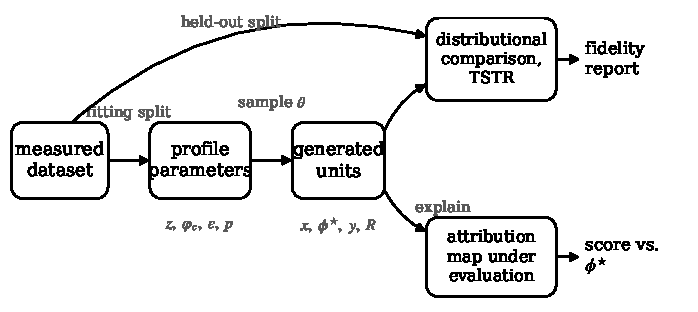
\includegraphics[width=0.8\linewidth]{img/fig_loop.pdf}
  \caption{Structure of the benchmark. Generator parameters are estimated from the fitting split of a measured dataset, giving a profile: the degradation state $z$, the channel mappings $\varphi_c$, the noise $\varepsilon$, and the inserted patterns $p$ (Section~\ref{sec:generator}). Drawing $\theta$ per unit generates units, each carrying the sequence $x$, the attribution ground truth $\phi^{\star}$, the decomposable target $y$, and the transfer target $R$ (Section~\ref{sec:target}). Attribution maps are scored on generated units only, since $\phi^{\star}$ is known nowhere else. The profile is separately compared against the held-out split, which took no part in fitting it.}
  \label{fig:loop}
\end{figure}
 
\subsection{Generator}
\label{sec:generator}
 
A generated unit consists of a multivariate sequence together with the targets and the attribution ground truth derived from it in Section~\ref{sec:target}. The sequence is $x \in \mathbb{R}^{T \times C}$, where $t \in \{1,\dots,T\}$ indexes positions and $c \in \{1,\dots,C\}$ indexes channels. In the datasets used here one position corresponds to one charge--discharge cycle, and $T$ is the position at which the unit reaches its end of life (EOL), defined in Equation~\ref{eq:state} below. Each channel is the sum of three terms,
\begin{equation}
  x_{t,c} \;=\; m_{t,c} \;+\; \sum_{k} p_{k,t,c} \;+\; \varepsilon_{t,c},
  \label{eq:generator}
\end{equation}
a mean component $m$, a set of inserted patterns $p_{k,t,c}$, and noise $\varepsilon$. Figure~\ref{fig:generator} shows the three terms and their sum for one channel. This composition, a base process into which patterns are inserted at recorded positions, is the design used by established synthetic benchmarks~\cite{tonekaboni2020,queen2023}. What differs is the role of the first term. There the base process is background, and the attribution ground truth does not depend on it; here the mean component carries the degradation trajectory and enters the target variable, which is what makes it graded rather than confined to the inserted patterns.
 
\begin{figure}[t]
  \centering
  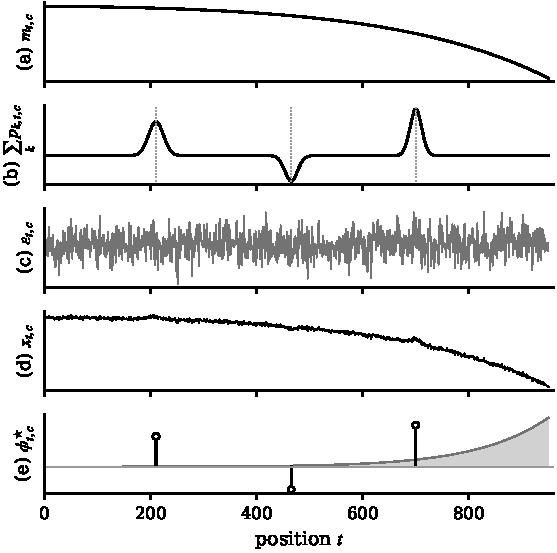
\includegraphics[width=0.6\linewidth]{img/fig_generator.pdf}
  \caption{One channel of a generated unit: (a) mean component, (b) inserted patterns, (c) noise, (d) their sum, which is what a model receives, and (e) the resulting attribution ground truth, a dense graded field (shaded) from the mean component and a sparse set of positions (stems) from the inserted patterns. Vertical scales are arbitrary.}
  \label{fig:generator}
\end{figure}
 
\subsubsection{Mean Component and Degradation State}
 
Degradation is one underlying process observed through several measured quantities, and those quantities do not follow the same shape: e.g., capacity falls while internal resistance and charge time rise. Fitting one parametric curve to every channel would impose a shape that only some of them have, while fitting an independent curve to each channel would instead leave the relationship between channels unconstrained. The generator therefore separates \emph{how far a unit has degraded} from \emph{what that degree of degradation looks like in a given channel}. The first is a scalar \emph{degradation state} $z_t$, the second a mapping $\varphi_c$ per channel,
\begin{equation}
  m_{t,c} \;=\; \varphi_c\!\left(z_t\right).
  \label{eq:mean}
\end{equation}
The mappings $\varphi_c$ are smooth, are shared across all units of a profile, and are fitted from the measured data as described in Section~\ref{sec:calibration}. Units therefore differ in the pace at which they age but not in what a given degree of ageing looks like: two units that have reached the same degradation state show the same expected values in every channel, at whatever positions they reached it. Figure~\ref{fig:mean} illustrates this for two units with different lifetimes. \rev{Because every channel is a function of the same degradation state, a channel that does not enter the target still carries that state, and whether a model relies on it cannot show whether the generated data leaks the target. Each profile therefore also contains two null channels with no dependence on the degradation state: one with a constant mapping plus noise, and one whose values are drawn from the measured values of a channel with unit identity and order removed by permutation. Both have zero weight in the target, and they are the channels on which leakage is tested (Section~\ref{sec:protocol}).}\revwhy{C2: null channels separate leakage from redundancy}
 
\paragraph{Definition of the degradation state and of EOL.}
Let $q_t$ denote the capacity channel, smoothed by a declared filter, \rev{let $q_{\mathrm{nom}}$ be the nominal capacity documented for the dataset, and let $q_1$ be the maximum of $q_t$ over a declared number $k$ of initial positions, attained at position $t_1$. EOL is reached when capacity has fallen to a fraction $\rho$ of nominal capacity, and the degradation state measures how much of the fall from $q_1$ to that threshold has been consumed,}
\begin{equation}
  \rev{z_t \;=\; \frac{q_1 - q_t}{q_1 - \rho\, q_{\mathrm{nom}}},}
  \qquad
  T \;=\; \min\{\, t \rev{\ge t_1} : z_t \ge 1 \,\}.
  \label{eq:state}
\end{equation}
The degradation state runs from $0$ at \rev{the early-life reference} to $1$ at EOL. Because both endpoints are fixed in advance, \rev{$\rho\, q_{\mathrm{nom}}$} by declaration and $q_1$ by observation, $z_t$ is a transform of the current capacity alone. It is therefore computable from data available up to $t$\rev{, once the first $k$ positions have been observed,} and $T$ is a consequence of the trajectory rather than an input to it. \rev{The early-life reference is a maximum over the first positions rather than the first value because measured capacity can rise over early cycles before it falls, and a first-position reference would make the degradation state negative over that interval; how often the two references differ is reported with the property audit of Section~\ref{sec:profiles}.}\revwhy{C3: EOL against nominal capacity; robust $q_1$}
The more obvious alternative—rescaling each unit's trajectory to the unit interval over its observed length—would make $z_t$ a function of $t/T$. In this case, the degradation state, and through Equation~\ref{eq:mean} every channel, would encode the unit's total lifetime at every position. Since total lifetime is what the transfer target of Section~\ref{sec:target} asks a model to predict,  the generated data would exhibit target leakage, and a model trained on it would depend on information that is unavailable at prediction time, a failure mode reported for RUL pipelines~\cite{mishchukaciids2026}.
 
Measured datasets do not agree on $\rho$. The common convention is a fall to $80\%$ of nominal capacity, but the experiments underlying some datasets were stopped at a fade of $20$ to $30\%$, and individual units within a dataset were carried to different final capacities. Adopting each dataset's own convention would define $z_t$ against a different endpoint in each profile and would render the parameter distributions fitted from them mutually incomparable. We therefore apply a single declared $\rho$ across all profiles\rev{, taken against the nominal capacity each dataset documents rather than against a unit's own initial capacity. The experiments stop cycling at thresholds stated relative to nominal capacity, so a fraction taken against a higher initial capacity would place EOL below the point at which cycling stopped and would exclude units for a reason unrelated to how they degrade. A unit whose early-life reference lies within a declared margin of the threshold is excluded, since the permitted fall is then too small to define the degradation state.} \rev{Some datasets were recorded only until capacity reached the stopping threshold, so a measured unit whose last recorded capacity lies within a declared tolerance of the threshold is taken to reach EOL at its last position, which is where the experiment itself located it; generated units are not truncated and follow Equation~\ref{eq:state} alone.}\revwhy{D13: records cut at the stopping rule} We report the number of units that never reach \rev{the threshold}, which are excluded \rev{from the quantities that depend on EOL (the parameter distribution, the length distribution, and the transfer target) and retained for those that do not (the channel mappings, the noise, and the inserted patterns), since their degradation state is defined}, and report the sensitivity of the fitted parameter distributions to $\rho$ across the range these conventions span\rev{, including the definition that takes $\rho$ against the first-position capacity}.
 
\paragraph{Shape of the degradation state.}
The trajectory $q_t$, and hence $z_t$, follows a parametric curve with a low-dimensional parameter vector $\theta$ drawn per unit from a distribution estimated from measured units. The functional form is not fixed in advance. Several established empirical fade models are fitted to each dataset and the one that fits best is selected, so that the shape carried by a profile is decided by the data it stands for rather than by us; Section~\ref{sec:calibration} gives the candidates and the selection rule.
 
\begin{figure}[t]
  \centering
  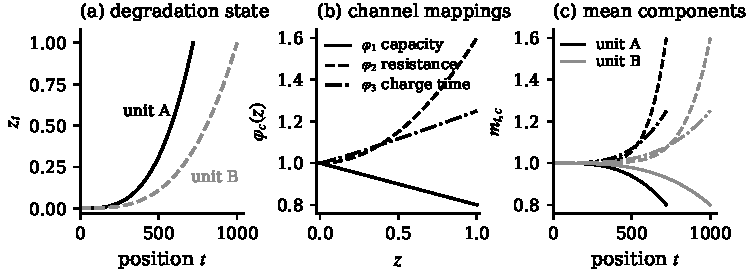
\includegraphics[width=0.75\linewidth]{img/fig_mean_component.pdf}
  \caption{Construction of the mean component. Two units advance through the degradation state at different paces and reach EOL at different positions (a). The same fitted mappings (b) are applied to both, giving mean components that differ in timing but not in the relationship between channels (c). Curves are illustrative.}
  \label{fig:mean}
\end{figure}
 
\subsubsection{Inserted Patterns and Noise}
 
\paragraph{Inserted patterns.}
Measured degradation trajectories are not smooth. Alongside the global degradation trend, capacity sequences carry local fluctuations, and the established works separates the two, decomposing the trajectory into a degradation trend, a regeneration component, and a residual fluctuation component~\cite{pan2022}. The positive fluctuations are \emph{capacity regeneration}: a temporary recovery of measured capacity that follows a rest period between cycles and persists over the cycles after it~\cite{qin2016,olivares2013}. Negative fluctuations follow from the conditions under which a cycle is measured rather than from the state of health of the cell; ambient temperature is the documented instance, entering prognostic models as an explicit input on the usable capacity of a cycle~\cite{olivares2013} and appearing as chamber temperature excursions in public cycling datasets~\cite{severson2019}. In both cases the deviation is treated as separate from the degradation trend, which is estimated and extrapolated in its own right~\cite{pan2022,qin2016}, and not as a change in how far the unit has degraded.
In this work, these fluctuations are incorporated as profiles without them would be smoother than the dataset they stand for, and the fidelity measurements would record the difference. They also supply the localized part of the attribution ground truth, which is the part the retrieval metrics reported on existing benchmarks are defined on.
The generator represents these effects as inserted patterns $p_{k,t,c}$, each described by a position, a signed amplitude, and a duration. Because they act on the observation and not on the degradation state, they do not alter $z_t$, the position of EOL, or the transfer target. Section~\ref{sec:calibration} states how they are detected in measured data and what is estimated from them. A profile enables only the inserted pattern types its dataset exhibits.
 
\paragraph{Noise.}
Noise is added per channel with variance and autocorrelation set during fitting, and has zero mean, $\mathbb{E}[\varepsilon_{t,c}] = 0$. Because retrieval scores depend on the signal-to-noise ratio, a generator cleaner than the measured data would report every attribution method as more accurate than it is.
 
\subsection{Targets and Attribution Ground Truth}
\label{sec:target}
 
Two quantities have to be distinguished. A \emph{target} is a value a model is trained to predict from a window of the sequence. The \emph{attribution ground truth} is the contribution that each position and channel of that window makes to the target; it is the quantity an attribution method is asked to recover and against which its output is scored. The generator defines two targets, for two different purposes. The \emph{decomposable target} $y$ is written down as an additive function of the generated components, so that its attribution ground truth follows from its form, and is the target used whenever attributions are scored. The \emph{transfer target} $R$ is the RUL, has a counterpart in every measured dataset, and is used only to test how well a profile reproduces the dataset it was fitted to.
 
\subsubsection{Decomposable Target and Attribution Ground Truth}
 
Let $W$ be a window of $L$ consecutive positions ending at position $t$, and let $u$ index the positions within it, $u \in \{t-L+1,\dots,t\}$. The decomposable target on that window is a weighted sum of the generated components:
\begin{equation}
  \rev{y \;=\; \sum_{(u,c)\,\in\, W} w_{u,c} \left( m_{u,c} - x^{0}_{c} \right) \;+\; \sum_{(u,c)\,\in\, W} w_{u,c} \sum_k p_{k,u,c}.}
  \label{eq:target}
\end{equation}

Since $m_{u,c} = \varphi_c(z_u)$, the first term is a fixed function of the degradation state over the window: $y$ summarises how far the unit has degraded across those positions, perturbed by whatever transients occurred in them. It is important to note that equation~\ref{eq:target} \emph{is not a physical law and is not proposed as a model of how RUL arises from a degradation trajectory}. The decomposable target is never compared against measured data, whereas the sequences and the transfer target are.
Because Equation~\ref{eq:target} is additive and written down rather than learned, the contribution of every position and channel is known exactly:
\begin{equation}
  \rev{\phi^{\star}_{u,c} \;=\; w_{u,c} \left( m_{u,c} - x^{0}_{c} \right) \;+\; w_{u,c} \sum_k p_{k,u,c}.}
  \label{eq:groundtruth}
\end{equation}

\rev{The first term of Equation~\ref{eq:groundtruth} is the graded field and the second the sparse set. Both are measured from the reference point $x^{0}_{c} = \varphi_c(0)$, the pristine level of channel $c$, which is declared per profile and identical across its units. It is the input at which the decomposable target is zero, so a unit that has not degraded and carries no inserted pattern has $y = 0$, and an attribution method whose values sum to the difference between the model output on the window and on its baseline recovers $\phi^{\star}$ only when that baseline is $x^{0}$ (Section~\ref{sec:models}), and a target measured from it can be reproduced by a map of the observed window, which a target containing the mean component itself cannot (see the reference model below). There is one weight per position and channel, $w_{u,c} = \kappa_c\, \pi_u$, the product of a channel factor and one of the position profiles below. The channel factor is zero on channels that do not enter the decomposable target and is declared in units of the degradation state on those that do, $\kappa_c = \beta_c / (\varphi_c(1) - \varphi_c(0))$, so that the full change of a channel between the pristine level and EOL contributes a declared share $\beta_c$ in every profile. Channel roles therefore differ in whether $\kappa_c$ is zero and whether the channel carries inserted patterns, not in the form of the weight. \rev{Every generated window is supplied together with its counterpart in which the inserted patterns are absent, and the two fields are scored on this pair: a method's attribution on the counterpart against the graded field, and the difference between its attributions on the window and on the counterpart against the sparse set, since for $\phi^{\star}$ these are exactly the two fields. Ranking the cells of a single map would not serve, because the graded field outweighs the patterns on the channel that carries them, so that even $\phi^{\star}$ would rank the sparse set last.} The position profile $\pi_u$ decides how the relevance of the mean component and of the inserted patterns is distributed across the positions of a window, and therefore what shape a correct attribution map has.}\revwhy{C1: one weight per cell about $x^0$; D01: paired scoring}


\rev{The weights cannot} be estimated from measurement: the purpose of $y$ is to be exactly decomposable so that the contribution of every observation follows from its form instead of being estimated; it has no counterpart in a measured dataset. Fitting the weights would require an external criterion, and both available criteria serve a different purpose. Deriving them from an attribution method applied to a trained model would make the attribution ground truth a function of one of the methods under evaluation. Fitting them so that $y$ approximates the transfer target would make $y$ a second estimate of a quantity the generator already records as a label. It is also indeterminate in the direction that matters: the mean component at adjacent positions within a window is close to collinear, so a fit pins down the aggregate weight far more tightly than its distribution across positions, which is what \rev{$\pi$} exists to specify. Fitted weights would also vary between profiles, making scores incomparable for the same reason $\rho$ is standardized.

Figure~\ref{fig:weights} shows the three weightings used. \emph{Recency} weighting increases smoothly toward the end of the window at a decay rate declared per profile; it keeps every position relevant while giving the field an ordering a method can be scored against. \emph{Uniform} weighting makes every position equally relevant; it is the limit in which no ordering exists to recover. \emph{Final-position} weighting places all weight on the last position; it is the opposite limit, in which \rev{both the graded field and the sparse set collapse into the last position of the window, so that an inserted pattern contributes only where it covers that position,} and it matches an explained model that reads only the last observation of a window. Reporting all three therefore measures how far a result depends on where relevance is placed rather than on which method produced it. The attribution methods under evaluation are scored against $\phi^{\star}$ under all three weightings, and we report whether the score orderings place the methods in the same sequence.

\begin{figure}[t]
  \centering
  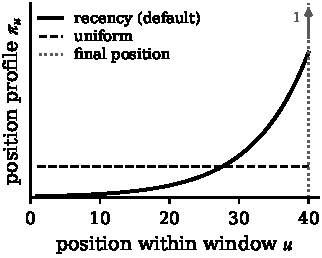
\includegraphics[width=0.35\linewidth]{img/fig_weights.pdf}
  \caption{Weighting of positions within a window. The recency weighting used by default keeps every position relevant while giving the graded attribution ground truth an ordering; the alternatives are degenerate in the two ways described in the text.}
  \label{fig:weights}
\end{figure}


 

\paragraph{Reference model.}
Attribution is evaluated on a trained model, so a low score may reflect error introduced by the attribution method or error in the model itself. To separate the two, the benchmark also provides a \emph{reference model}: \rev{the affine map $g(x) = \sum_{(u,c)\in W} w_{u,c}\,(x_{u,c} - x^{0}_{c})$, which applies the weights $w$ to the deviation of the observed window from the reference point. It reproduces the target exactly when noise is absent and otherwise differs from it only through $\sum_{(u,c)\in W} w_{u,c}\,\varepsilon_{u,c}$, whose expectation is zero since $\mathbb{E}[\varepsilon]=0$. Its intercept does not enter attributions computed from the reference point. Because the map is affine} and its weights are known, attributions computed for it can be compared against an analytically available solution, and any remaining error is attributable to the attribution method alone. The reference model addresses the model and not the target: it establishes what an attribution method achieves when the model is exactly right, and says nothing about whether the target is well chosen, which is what the two properties above report.
 
\subsubsection{Transfer Target}
 
The decomposable target has no counterpart in a measured dataset, so a model trained to predict it cannot be evaluated on measured data. The generator therefore records a second label, the RUL at position $t$,
\begin{equation}
  R_t \;=\; T - t,
  \label{eq:transfer}
\end{equation}
with $T$ as defined in Equation~\ref{eq:state}. This is the same quantity that measured datasets provide as a RUL label. It is used only for the transfer measurement of Section~\ref{sec:protocol} and forms no part of the attribution ground truth.
 
Two points follow from Equation~\ref{eq:transfer}. First, $R$ is not a function of $z_t$: two units that have reached the same degradation state have different RUL according to how fast they are advancing through it. This is what makes the transfer measurement informative, since a profile whose fitted parameter distribution advances units at the wrong pace will fail it even when the generated sequences match the measured ones in distribution. Second, $R$ depends on the whole trajectory and is therefore a label and never an input. Neither $R$, nor $T$, nor any quantity derived from them is available to a model at prediction time, a restriction stated in full in Section~\ref{sec:calibration}.
 
\subsection{Fitting the Generator to a Measured Dataset}
\label{sec:calibration}
 
A \emph{profile} is the set of generator parameters obtained from one measured dataset. Fitting uses the training split only, so that the units later used to assess the profile take no part in producing it. The procedure has six steps.
 
\emph{First}, the capacity channel is extracted for every unit\rev{, readings that no degradation process produces are removed (\rev{in any channel,} a single position departing from its neighbourhood by more than a declared fraction of \rev{its typical value}, which the detection rule below could never admit as a pattern, and readings below half of nominal capacity from which the record later recovers),} and \rev{the series is} smoothed by a Savitzky–Golay filter, and EOL is located by Equation~\ref{eq:state}. \emph{Second}, candidate parametric families are fitted to each unit's capacity trajectory \rev{from the early-life reference to EOL} by nonlinear least squares. The families considered are the two-term exponential established for capacity fade~\cite{he2011}, a rollover form whose parameters are the initial rate, the transition position, the transition width, and the terminal rate~\cite{saxena2022}, and a power law, which has fewer parameters but cannot express a transition. The family is selected per dataset by cross-validated fit error across units\rev{, among the families whose parameters are determined by the data rather than held at a bound of their range in more than a declared share of units, and a family with fewer parameters is preferred within a declared margin of the lowest error}; the error of every candidate is reported.\revwhy{D04: identified families only} The empirical distribution of the fitted parameters over units is the profile's distribution of $\theta$. \emph{Third}, the mappings $\varphi_c$ of Equation~\ref{eq:mean} are fitted as smooth monotone functions of the fitted degradation state, and the covariance among channels is recorded; for the capacity channel the mapping is affine by construction, since Equation~\ref{eq:state} defines the degradation state as an affine transform of that channel\rev{, and it is taken at the median early-life reference of the fitting units so that it is shared across units like every other mapping}. \emph{Fourth}, the residuals of the trajectory fit supply the noise variance and autocorrelation, computed with the positions occupied by detected patterns excluded, so that transients are not counted as noise. \emph{Fifth}, the same residuals supply the inserted patterns, by the detection procedure stated below. \emph{Sixth}, the empirical distribution of unit lengths is recorded.
 
The distinction between what is measured and what is chosen is reported explicitly, since it determines what the benchmark can claim. Estimated from the measured dataset are the distribution of $\theta$, the choice of family, the mappings $\varphi_c$ and the covariance among channels, the noise variance and autocorrelation, the rate, amplitude, and duration of the inserted patterns, and the length distribution. Declared by design are the EOL fraction $\rho$, \rev{the nominal capacity of each dataset as documented, the number $k$ of positions over which the early-life reference is taken and the margin below which a unit is excluded,} \rev{the fraction of nominal capacity beyond which a single reading is removed, the tolerance within which a truncated record reaches EOL, the share of units at a parameter bound beyond which a family is not eligible and the margin within which a simpler family is preferred, the factor by which a pattern type must exceed its noise-only rate, the minimum counts per measurement,} the smoothing window length and polynomial order, the pattern detection thresholds, the number of channels and which of them enter the target, \rev{the channel shares $\beta_c$ and position profiles of the weights $w$, the definition of the reference point $x^{0}$,} the window length $L$, and the generator settings varied in the protocol.
 
\paragraph{Detecting the inserted patterns and estimating their parameters.}
Two families of detection procedure are established in battery prognostics. The first tests the residual of a fitted degradation trend for a departure the trend does not account for, either by a statistical test on the residual sequence~\cite{ma2021} or by decomposing the sequence and assigning the components uncorrelated with the trend to regeneration~\cite{pan2022}. The second triggers on the rest time between adjacent cycles, on the mechanism that a rest longer than a threshold produces a regeneration over the cycles that follow~\cite{qin2016,olivares2013}. We adopt the first. Rest time is recoverable from the timestamps of some public datasets and not of others, whereas the residual of the trajectory fit is available for every dataset by step two above, and the same rule has to apply to every profile for the fitted parameters to be comparable across them.

The rule is as follows. A candidate pattern is a run of consecutive positions whose residual from the fitted trajectory exceeds a declared multiple of the residual scale and whose length reaches a declared minimum \rev{without exceeding the smoothing window}; the sign of the run gives the type. \rev{A departure that lasts longer than the smoothing window survives smoothing, so it is part of the smoothed capacity and changes the degradation state, which an inserted pattern must not do; it therefore belongs to the mean component.}\revwhy{D16: patterns cannot move $z_t$} For each detected pattern we record the position of its extremum, its signed amplitude, and its duration in positions, and we estimate the distribution of amplitude and of duration together with the per-unit rate of occurrence over the dataset. Amplitude and duration are the quantities the rest-time literature also extracts from measured sequences, as the value reached at the regeneration cycles and the number of cycles the regeneration region spans~\cite{qin2016}, so the fitted distributions are comparable with published characterizations of the same phenomenon~\cite{qin2016,olivares2013}.

The procedure has two thresholds, and both are declared before fitting and reported with the counts they produce, because the estimated distributions are not insensitive to them: a multiple set too low absorbs noise into the pattern distributions, inflating the rate and biasing the amplitude distribution downward, while one set too high empties them. We therefore report the detected rate and the amplitude distribution over a declared range of the multiple, alongside the residual scale itself, and a type is enabled in a profile only \rev{if the rule detects it at least a declared factor more often than in noise simulated with the profile's own fitted variance and autocorrelation, since detections that the fitted noise alone produces are the noise the threshold exists to exclude; a type not detected beyond that rate is not enabled} rather than being generated at an assumed rate.\revwhy{D05: enable only above the noise rate}
 
\paragraph{Splitting and use of future information.}
Windows drawn from one unit are strongly dependent, so all splits are performed at the level of units rather than windows, on both generated and measured data. Normalization statistics are computed on training units alone. No input feature may be derived from a quantity that depends on positions after $t$ or on the full length of a sequence, since that length is the label; in particular the normalized position $t/T$ is excluded while the elapsed position $t$ is not. This restriction applies to model inputs. It does not apply to the fitting procedure above, which is not a model and is allowed to use each measured unit in full, nor to the targets, which are labels.
 
\subsection{Profiles}
\label{sec:profiles}
 
Three profiles are built. \textbf{MATR}~\cite{severson2019} supplies the largest number of units and is the profile against which the fidelity measurements are primarily read; it also supplies the reference channel set, recording discharge capacity, internal resistance, charge time, and temperature statistics per cycle. \textbf{HUST}~\cite{ma2022hust} contains cells of the same chemistry and format cycled under different discharge protocols in a different laboratory, and therefore tests whether the fitting procedure transfers when the cell is held fixed and the protocol is not. \textbf{NASA PCoE}~\cite{saha2007} is the smallest of the three and is included for one property the others lack: documented capacity regeneration, without which the corresponding pattern type cannot be fitted from measurement. Its fidelity measurements are reported with the number of units it contains, since that number limits what they can establish.
 
Before a profile is built, the property it is included for is verified on the data rather than taken from the literature. We report the fraction of units whose smoothed capacity channel is monotone within tolerance, the detected rate and amplitude of capacity regeneration, the fraction of units reaching the declared EOL threshold\rev{, how often the early-life reference differs materially from the first-position capacity}, the distribution of unit lengths, and which channels are available across all units. A dataset that does not exhibit the property it was selected for has its role reassigned or is dropped, and the outcome is reported.
 
\subsection{Evaluation Protocol}
\label{sec:protocol}
 
\subsubsection{Profile Fidelity}
 
The first research question asks how closely each profile reproduces the dataset it was fitted to. Three measures established in the generative time-series literature are reported per profile: the classification error of a discriminator trained to separate generated from measured windows~\cite{yoon2019}, a Fr\'{e}chet-style distance computed in a learned representation space~\cite{psagan2022}, and the agreement of the cross-channel covariance structure. All three are computed on windows, with the window length and the effective number of independent units stated alongside. \rev{Every measurement in the protocol has a declared minimum number of units or events, set so that its resampling interval does not extend beyond half of its value on either side; a measurement below its minimum is reported as void with its count, following the convention of the usability checks.}\revwhy{D02: minimum counts per use}
 
The discriminative measure is reported as a coarse indicator only. On sequences of the lengths considered here, a discriminator separates the two sources whenever any property is mismatched, and its error saturates without indicating which property is responsible. The property-level comparisons therefore carry the evidence: the fitted distribution of $\theta$, the noise variance and autocorrelation, the length distribution, the rate and amplitude of capacity regeneration, and the cross-channel covariance are each reported for the generated and the measured side.
 
The transfer measurement follows the TSTR procedure~\cite{esteban2017} and is shown in Figure~\ref{fig:tstr}. A model is trained on a profile using the transfer target of Equation~\ref{eq:transfer}, and is evaluated on units of the paired dataset that took no part in fitting the profile, using their RUL label. The same architecture trained on the measured units of the fitting split, and evaluated on the same held-out units, gives the reference. We report the ratio of the two errors with a bootstrap interval rather than the absolute error, which is not comparable across datasets with different lifetime ranges. A ratio near one indicates that a model learns as much from the profile as from the dataset it stands for. Each profile is evaluated against its own paired dataset only, since a pooled evaluation would allow a close match on one dataset to compensate for a poor match on another.
 
\begin{figure}[t]
  \centering
  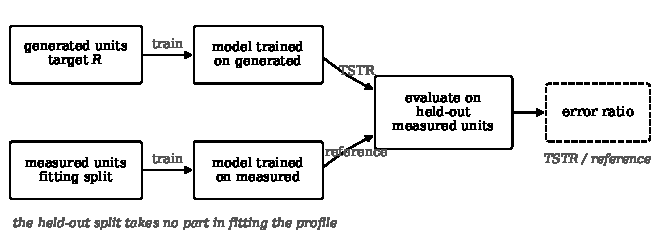
\includegraphics[width=0.8\linewidth]{img/fig_tstr.pdf}
  \caption{The transfer measurement. Two models are trained, one on a profile and one on the measured units used to fit it, and both are evaluated on measured units held out from fitting. The reported quantity is the ratio of their errors.}
  \label{fig:tstr}
\end{figure}
 
\subsubsection{Usability of the Attribution Ground Truth}
 
The second research question asks whether the attribution ground truth is usable, which requires that a model can learn the decomposable target and that the two kinds of contribution can be told apart. Four checks are reported, alongside the two properties of the target declared in Section~\ref{sec:target}. A model must reach a predetermined accuracy on each profile before any attribution is computed on it; scores obtained below that threshold are reported as void rather than as poor. The correlation between the graded and the sparse contribution fields across the dataset must remain below a declared bound, so that a method is not credited for recovering one when it has recovered the other. Retraining with each of the two terms of Equation~\ref{eq:target} removed in turn must change model behaviour in the direction the construction predicts, confirming that both are used. Finally, permutation importance must show that models do not rely on \rev{the null channels of Section~\ref{sec:generator}; since these carry no degradation state by construction,} a model that does indicates that the generated data leaks the target through a channel intended to be irrelevant, and the profile is corrected before use. \rev{Channels that carry the degradation state but have zero target weight are not held to the same bound, since a model may read the state from them as legitimately as from the channels that enter the target. For each of them we report how well it is predicted from the remaining channels and its importance when it is permuted conditionally on them, which is near zero when the channel is redundant and positive only when it carries information the other channels do not.}
 
\subsubsection{Responsiveness of the Scores}
 
The third research question asks whether the scores distinguish better from worse attribution maps, and over which generator settings they continue to do so. The first part is measured without involving any attribution method. The ground-truth field itself is a correct attribution map by construction, so it can be degraded in controlled amounts: adding noise of increasing variance, shifting a known fraction of the mass toward the start or the end of the sequence, smoothing across neighbouring positions, and randomly permuting a known fraction of the values. A score that does not decrease as the map is degraded is not measuring what it is intended to measure, and the smallest degradation that a score resolves reliably is reported as its resolution.
 
The second part varies the generator settings that control task difficulty: noise variance, the sharpness of the transition in the degradation state, sequence length, and the amplitude of the inserted patterns. Scores that saturate near their maximum indicate a task too easy to separate methods, and scores near chance indicate one that is too hard. The range over which they remain responsive is reported as the operating range of the benchmark, so that later use does not extend beyond the settings for which the measurements were shown to be informative.
 
\subsection{Models and Baselines}
\label{sec:models}
 
Attribution is evaluated on a single trained architecture, a recurrent network with long short-term memory units, together with the reference model of Section~\ref{sec:target}. The benchmark scores attribution maps against known contributions and is independent of the model used to produce them, so a second trained architecture would not contribute to the three research questions; the reference model provides the comparison that removes model error, which a second trained model provides only indirectly. \rev{The two columns differ in kind, and the reference model is the primary scoring target. Its function is known, so $\phi^{\star}$ is its faithful attribution and its column measures the attribution method. The channels of a window share one degradation state, so many functions of the window reproduce the decomposable target equally well, and an accurate trained model need not implement the one that defines $\phi^{\star}$; its column therefore also reflects which of these functions the model learned. To bound that effect, an ensemble of equally accurate models differing in initialization and size is trained, and the spread of their scores is reported beside the scores of each method as the limit it places on any method.}\revwhy{C2: ground truth not identifiable for a trained model}
 
Three published methods are run at their default configurations on both the trained and the reference model: TimeSHAP~\cite{bento2021} for perturbation-based Shapley attribution over sequences, Integrated Gradients (IG)~\cite{sundararajan2017} for gradient-based attribution, and feature occlusion~\cite{suresh2017}. Methods that optimise a mask per instance~\cite{crabbe2021,enguehard2023,liu2024} are excluded, since their scores depend on hyperparameters whose tuning is a comparison of methods rather than a reference measurement. These results are reported as reference values for later work rather than as an evaluation of the methods themselves. Accordingly, they are reported in aggregate, without stratification by position within the trajectory and without a diagnosis of the causes of any differences observed.

\rev{Each of the three methods computes attributions relative to a baseline, and Shapley-based and path-based attributions sum to the difference between the model output on the window and on that baseline. Scoring them against $\phi^{\star}$ therefore presumes that the model output on the baseline is zero, which holds for the reference model only at the reference point $x^{0}$. The declared baseline is accordingly the pristine window, every position of which is at $x^{0}$: it is the Integrated Gradients baseline, the occlusion value, and the TimeSHAP background instance. Unlike a zero input, the pristine window lies close to the first windows of every unit, so the trained model is not queried on a window unlike any it was trained on. Because the decomposable target is affine with known weights, the attribution ground truth from any other baseline $b$ is $w_{u,c}\,(m_{u,c} + \sum_k p_{k,u,c} - b_{u,c})$, and the benchmark supplies it, so a method run from a different baseline is scored against the ground truth that matches it and methods can still be run at their defaults. TimeSHAP is additionally run from the average event it uses by convention, as a readout of whether the ordering of the reference values depends on the baseline. A background conditioned on the local mean component is not adopted as the reference, although it is natural on a drifting channel, since it would make trend-conditional backgrounds correct by construction and any later evaluation of such backgrounds circular. Occlusion satisfies no efficiency property, so its values are compared with $\phi^{\star}$ in rank and retrieval but not in sum.}\revwhy{C4: declared baseline; ground truth per baseline}
 
Generation, model initialization, and any sampling performed by an attribution method are controlled by separate random seeds, so that the contribution of each to the variance of a score can be reported separately. The generator, the fitted profile parameters, the seeds, the trained and reference models, the ground-truth fields, and the scoring code are made available as stated in Section~1.

\section{Results}
\label{sec:results}

This section reports the measurements defined in Section~\ref{sec:protocol}, one subsection per research question, followed by the reference values of Section~\ref{sec:protocol} for published attribution methods. \hl{All entries below are placeholders: the tables and figures state what is reported and in what form, and no value in them has been measured yet.} Every reported quantity is accompanied by an interval obtained by bootstrap over units, and the seeds controlling generation, model initialization, and attribution sampling are varied separately so that their contributions to the spread are reported apart.

\subsection{Profile Fidelity}
\label{sec:res:fidelity}

Table~\ref{tab:res:fidelity} reports, per profile, the discriminative measure, the representation-space distance, the agreement of the cross-channel covariance structure, and the transfer ratio, with the window length and the effective number of independent units stated alongside. The discriminative measure is read as a coarse indicator only, for the reason given in Section~\ref{sec:protocol}; the property-level comparison of Table~\ref{tab:res:properties} carries the evidence, setting the generated and the measured side of each fitted quantity against each other. Figure~\ref{fig:res:fidelity} shows the fitted and the measured capacity trajectories of the same profile for visual comparison, which is reported as illustration and not as a measurement.

\begin{table}[t]
  \caption{Profile fidelity. One row per profile. The transfer ratio is the error of a model trained on the profile divided by that of the same architecture trained on the measured fitting split, both evaluated on the held-out measured units; a ratio near one indicates that a model learns as much from the profile as from the dataset it stands for. \hl{Placeholder values.}}
  \centering
  \begin{tabular}{lccccc}
    \toprule
    Profile & Units (eff.) & Discriminative err. & Repr. distance & Covariance agr. & Transfer ratio [CI] \\
    \midrule
    MATR & -- & -- & -- & -- & -- [--, --] \\
    HUST & -- & -- & -- & -- & -- [--, --] \\
    NASA PCoE & -- & -- & -- & -- & -- [--, --] \\
    \bottomrule
  \end{tabular}
  \label{tab:res:fidelity}
\end{table}

\begin{table}[t]
  \caption{Property-level comparison between each profile and the dataset it was fitted to. Each cell holds the measured value and the generated value of the same quantity. The detection thresholds behind the regeneration rows, and the sensitivity of those rows to them, are reported with the counts of Section~\ref{sec:calibration}. \hl{Placeholder values.}}
  \centering
  \begin{tabular}{lcccccc}
    \toprule
    & \multicolumn{2}{c}{MATR} & \multicolumn{2}{c}{HUST} & \multicolumn{2}{c}{NASA PCoE} \\
    \cmidrule(r){2-3} \cmidrule(r){4-5} \cmidrule(r){6-7}
    Property & meas. & gen. & meas. & gen. & meas. & gen. \\
    \midrule
    Trajectory family, fit error & -- & -- & -- & -- & -- & -- \\
    Drift rate & -- & -- & -- & -- & -- & -- \\
    Transition position & -- & -- & -- & -- & -- & -- \\
    Noise variance (per channel) & -- & -- & -- & -- & -- & -- \\
    Noise autocorrelation & -- & -- & -- & -- & -- & -- \\
    Unit length & -- & -- & -- & -- & -- & -- \\
    Regeneration rate & -- & -- & -- & -- & -- & -- \\
    Regeneration amplitude & -- & -- & -- & -- & -- & -- \\
    Regeneration duration & -- & -- & -- & -- & -- & -- \\
    Cross-channel covariance & -- & -- & -- & -- & -- & -- \\
    \bottomrule
  \end{tabular}
  \label{tab:res:properties}
\end{table}

\begin{figure}[t]
  \centering
  \fbox{\parbox[c][3.0cm][c]{0.9\linewidth}{\centering \texttt{[FIGURE]} Measured and generated capacity trajectories of one profile, one panel per profile: measured units in the background, units generated from the fitted parameter distribution overlaid, with the state axis of Equation~\ref{eq:state} marked.}}
  \caption{Fitted against measured trajectories, reported as illustration alongside the measurements of Tables~\ref{tab:res:fidelity} and~\ref{tab:res:properties}.}
  \label{fig:res:fidelity}
\end{figure}

\subsection{Usability of the Attribution Ground Truth}
\label{sec:res:usability}

Table~\ref{tab:res:usability} reports the four checks of Section~\ref{sec:protocol} together with the two declared properties of the decomposable target. A profile that fails the accuracy threshold has its attribution scores reported as void rather than as poor, and the row records which of the two outcomes applies; the same convention is used in every table that follows.

\begin{table}[t]
  \caption{Usability of the attribution ground truth, per profile. The first two rows are the declared properties of the decomposable target, the remaining rows the checks that the target is learnable and that its two contributions are separable. Each threshold or declared bound is stated in the row it governs. \hl{Placeholder values.}}
  \centering
  \begin{tabular}{llccc}
    \toprule
    Quantity & Bound & MATR & HUST & NASA PCoE \\
    \midrule
    Variance ratio of the two terms of Eq.~\ref{eq:target} & band \hl{--} & -- & -- & -- \\
    Association of $y$ with RUL & reported & -- & -- & -- \\
    Model error on $y$ & $\le$ \hl{--} & -- & -- & -- \\
    Correlation of graded and sparse fields & $\le$ \hl{--} & -- & -- & -- \\
    Error change, mean term removed & sign & -- & -- & -- \\
    Error change, pattern term removed & sign & -- & -- & -- \\
    Permutation importance, zero-weight channels & $\approx 0$ & -- & -- & -- \\
    \bottomrule
  \end{tabular}
  \label{tab:res:usability}
\end{table}

\subsection{Responsiveness of the Scores}
\label{sec:res:responsiveness}

The first part of the third research question is measured without any attribution method, by degrading the attribution ground-truth field itself in controlled amounts. Figure~\ref{fig:res:degradation} plots each score against the magnitude of each degradation, and Table~\ref{tab:res:resolution} reports, per score and per degradation, the smallest magnitude the score resolves reliably. The second part varies the generator settings that control task difficulty; Figure~\ref{fig:res:range} plots the scores against each setting, and the range over which they remain responsive is reported in Table~\ref{tab:res:range} as the operating range of the benchmark.

\begin{figure}[t]
  \centering
  \fbox{\parbox[c][3.4cm][c]{0.9\linewidth}{\centering \texttt{[FIGURE]} Each score against degradation magnitude, one panel per degradation operator: added noise, mass shifted toward the start or the end of the sequence, smoothing across neighbouring positions, and a permuted fraction of the values. Rank agreement against the graded field and retrieval metrics against the sparse set are drawn as separate series.}}
  \caption{Score response to controlled degradation of a correct attribution map.}
  \label{fig:res:degradation}
\end{figure}

\begin{table}[t]
  \caption{Resolution of each score: the smallest degradation magnitude that is resolved reliably, per degradation operator, with the criterion for reliability stated in Section~\ref{sec:protocol}. \hl{Placeholder values.}}
  \centering
  \begin{tabular}{lcccc}
    \toprule
    Score & Added noise & Shifted mass & Smoothing & Permuted fraction \\
    \midrule
    Rank agreement, graded field & -- & -- & -- & -- \\
    Retrieval, sparse set & -- & -- & -- & -- \\
    \bottomrule
  \end{tabular}
  \label{tab:res:resolution}
\end{table}

\begin{figure}[t]
  \centering
  \fbox{\parbox[c][3.4cm][c]{0.9\linewidth}{\centering \texttt{[FIGURE]} Each score against the generator settings that control task difficulty, one panel per setting: noise variance, sharpness of the transition in the degradation state, sequence length, and amplitude of the inserted patterns. Saturation near the maximum of a score and values near chance are both marked.}}
  \caption{Score response to the generator settings, from which the operating range of Table~\ref{tab:res:range} is read.}
  \label{fig:res:range}
\end{figure}

\begin{table}[t]
  \caption{Operating range of the benchmark: the interval of each generator setting over which the scores remain responsive, outside which later use is not supported by these measurements. \hl{Placeholder values.}}
  \centering
  \begin{tabular}{lccc}
    \toprule
    Setting & Range examined & Responsive range & Failure mode outside it \\
    \midrule
    Noise variance & -- & -- & -- \\
    Transition sharpness & -- & -- & -- \\
    Sequence length & -- & -- & -- \\
    Pattern amplitude & -- & -- & -- \\
    \bottomrule
  \end{tabular}
  \label{tab:res:range}
\end{table}

\subsection{Reference Values for Published Methods}
\label{sec:res:reference}

Table~\ref{tab:res:methods} reports the three methods of Section~\ref{sec:protocol} at their default configurations, on the trained architecture and on the reference model of Section~\ref{sec:target}. These are reference values for later work rather than an evaluation of the methods themselves, and are therefore reported in aggregate, without stratification by position within the trajectory and without a diagnosis of the causes of any differences observed. The difference between the two columns of each pair is the part of a score attributable to the model rather than to the attribution method, since the reference model reproduces the decomposable target up to $\varepsilon$.

\begin{table}[t]
  \caption{Reference values per attribution method, on the trained model and on the reference model, averaged over profiles that pass the usability checks of Table~\ref{tab:res:usability}. Rank agreement is measured against the graded field, retrieval against the sparse set, and mass on zero-weight channels is error by construction. \hl{Placeholder values.}}
  \centering
  \begin{tabular}{llcccccc}
    \toprule
    & & \multicolumn{2}{c}{Rank agreement} & \multicolumn{2}{c}{Retrieval} & \multicolumn{2}{c}{Zero-weight mass} \\
    \cmidrule(r){3-4} \cmidrule(r){5-6} \cmidrule(r){7-8}
    Method & Family & trained & ref. & trained & ref. & trained & ref. \\
    \midrule
    TimeSHAP & perturbation & -- & -- & -- & -- & -- & -- \\
    IG & gradient & -- & -- & -- & -- & -- & -- \\
    Feature occlusion & occlusion & -- & -- & -- & -- & -- & -- \\
    \bottomrule
  \end{tabular}
  \label{tab:res:methods}
\end{table}

\section{Discussion and future work}

\paragraph{\rev{What the benchmark can adjudicate.}}
\rev{The attribution ground truth is a property of the function that defines the decomposable target, not of the data alone. For the reference model that function is the model, so channel- and position-level ground truth is identifiable and a score measures the attribution method. For a trained model it is not: the channels share one degradation state, several functions of a window reproduce the target equally well, and a faithful attribution of the function a model actually learned can differ from $\phi^{\star}$. Scores on trained models therefore carry the model's own choice among equivalent functions, and the ensemble spread reported with them marks how much of a difference between methods that choice can account for.}

\subsection{Future work}
\paragraph{Learned component models.}
The generator fixes three components and a parametric family for each, which bounds the shapes a profile can express. A natural extension is to learn the components instead, with a model emitting a smooth, a localized, and an unstructured part that sum to the sequence. The attribution ground truth is unaffected, since it requires only that the generator record which part of each value it produced, not that the split be recovered from measurement; realism of $x$ would improve while the answer key stays exact. The three roles would have to be retained, as the graded and sparse measures and the exclusion of noise are defined against them, and the present benchmark would serve to validate such a model, since it is where a known decomposition exists to recover.

\section{Conclusion}
Your conclusion here

\section*{Acknowledgments}
This research was co-funded by the European Union HORIZON TMA MSCA Doctoral Networks / HORIZON-MSCA-2023-DN-01 / project TUAI / grant agreement N° 101168344. Views and opinions expressed are, however, those of the author(s) only and do not necessarily reflect those of the European Union or the European Research Executive Agency. Neither the European Union nor the granting authority can be held responsible for them. Co-funded by the Statutory Research funds of the Department of Distributed Systems and Informatic Devices, Silesian University of Technology, Gliwice, Poland (Grants BK-244/RAu8/2025 02/110/BK\_25/1036).

During the preparation of this manuscript, the authors used Anthropic Claude Opus 5 for the purposes of readability improvement, proofreading, and assisting with code implementation. The authors have reviewed and edited the output and take full responsibility for the content of this publication.

%Bibliography
\bibliographystyle{unsrtnat}  
\bibliography{references}  


\end{document}